\documentclass[pdf]{beamer}

\usepackage{graphicx}
\usepackage[dvipsnames]{xcolor}
\usepackage{subfig}

\mode<presentation>{}

\usetheme{Rochester}

\setbeamertemplate{caption}{\insertcaption}
\captionsetup[subfloat]{labelformat=empty}

\title{A good programming language is a \textit{Functional} one}
\author{Artin Ghasivand}
\titlegraphic{
  \centering
  
\includegraphics[width=0.10\linewidth]{CS-talks}
}

\newcommand{\code}[1]{\textcolor{Red}{\textsf{#1}}}

\begin{document}

\begin{frame}
  \titlepage
\end{frame}

\section{Models of Computation}
\label{sec:models-of-computation}

\begin{frame}{People}
  \begin{figure}[ht!]
    \centering
    \subfloat[Alonzo Church]{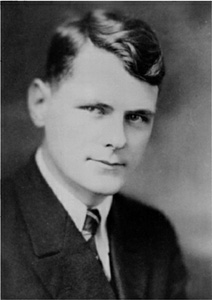
\includegraphics[width=0.30\linewidth]{Alonzo-Church}}
    \hspace{0.1cm}
    \subfloat[Kurt Gödel]{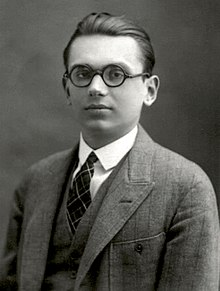
\includegraphics[width=0.30\linewidth]{Kurt-Godel}}
    \hspace{0.1cm}
    \subfloat[Alan Turing]{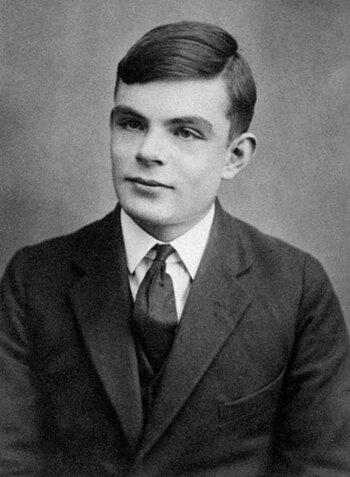
\includegraphics[width=0.30\linewidth]{Alan-Turing}}
  \end{figure}
  \begin{itemize}
  \item Alonzo Church: Untyped Lambda-Calculus, 1935
  \item Kurt Gödel: General Recursive functions, 1935 (written down by his student, Stephen Kleene)
  \item Alan Turing: Turing machines, 1936
  \end{itemize}
\end{frame}

\begin{frame}{Untyped Lambda-Calculus}
Syntax of the untyped lambda-calculus
  \begin{figure}[H]
    \centering
    \begin{tabular}{c c l l}
      $var$  & $\ni$   & $a,b,ab,..$         & Variable names  \\
      $term$ & $::=$ & $var$               & Variable \\
             & $|$   & $\lambda var. term$       & Abstraction \\
             & $|$   & $term_1 \: term_{2}$ & Application \\
    \end{tabular}
  \end{figure}
\end{frame}

\begin{frame}{Untyped Lambda-Calculus extended with natural numbers}
  Syntax of
    \begin{figure}[H]
    \centering
    \begin{tabular}{c c l l}
      $num$  & $\ni$   & $0,1 ...$           & Natural numbers \\
      $var$  & $\ni$   & $a,b,ab,..$         & Variable names  \\
      $term$ & $::=$ & $var$               & Variable        \\
             & $|$   & $\lambda var. term$       & Abstraction    \\
             & $|$   & $term_1 \: term_{2}$ & Application     \\
    \end{tabular}
    \end{figure}

    Assume the plus operator $+$ is a builtin function:
    \begin{figure}
    \begin{tabular}{l}
      $y$ \\

      $\lambda x. \: x$ \\
      $\lambda x. \: x + 2$ \\
      $\lambda x. \: \lambda y. \: x$ \\

      $(\lambda x. x + 2) \: 2$ \\
      $(\lambda x. x) \: 2$ \\
    \end{tabular}
  \end{figure}
\end{frame}

\begin{frame}{Untyped Lambda-Calculus: Reduction}
  \begin{itemize}
  \item The process of evaluating terms is called \emph{reducing} them
  \item Reducing $(\lambda x. x + 2) \: 2$ will give us \emph{4}
  \item The formal name for this process is called \textit{beta-reduction}
  \end{itemize}
\end{frame}

\begin{frame}{Untyped Lambda-Calculus: Currying}
  \begin{itemize}
  \item Lambda abstractions can only take \emph{one} argument
  \item Multiple argument functions are encoded as functions that return \emph{functions}
  \item Application is \emph{left associative}: $fun \: arg_{1} \: arg_{2}$ is the same as $(fun \: arg_{1}) \: arg_{2}$
  \end{itemize}

  Example: \code{$f(x,y) = x + y$} is encoded as \code{$\lambda x. \: (\lambda y. \: x + y)$}.

  \begin{itemize}
  \item $(\lambda x. \: (\lambda y. \: x + y)) 5$ reduces to $\lambda y. \: 5 + y$
  \item $(\lambda x. \: (\lambda y. \: x + y)) 5 9$ reduces to $5 + 9$
  \end{itemize}

\end{frame}

\begin{frame}{Untyped Lambda-Calculus: Meaningless terms}
  What is the meaning of the following examples?
  \begin{itemize}
  \item 3 3 (we are applying 3 to 3)
  \item 9 $\lambda x. \: x$
  \item $(\lambda x. \: x) (\lambda y. \: y)$
  \end{itemize}
  Answer: They \textbf{Don't} have one!

  In a programming language like Python, such terms result in a \textbf{runtime error}!
\end{frame}

\begin{frame}{Simply Typed Lambda-Calculus}
The syntax of Simply Typed Lambda-Calculus extended with natural numbers
  \begin{figure}[H]
    \centering
    \begin{tabular}{c c l l}
      $tyvar$ & $\ni$   & $\alpha, \beta, ...$  & Type variable \\
      $num$   & $\ni$   & $0,1 ...$    & Natural numbers \\
      $var$   & $\ni$   & $a,b,ab,..$  & Variable names  \\

      $Type$  & $::=$ & $tyvar$        & Type variable \\
              & $|$   & $\mathbb{N}$            & Natural number \\
              & $|$   & $Type \to Type$  & Function       \\

      $term$  & $::=$ & $var$                          & Variable   \\
              & $|$   & \code{$\lambda var : Type. \: term$} & Abstraction \\
              & $|$   & $term_1 \: term_{2}$           & Application   \\
              & $|$   & $num$                         & Natural number \\
    \end{tabular}

  \end{figure}

\end{frame}

\begin{frame}{Simply Typed Lambda-Calculus}
  For our purposes, you can think of a \textit{type} as classifier for \textit{terms}. But remember a term \textit{can't have multiple types!}.
  Examples:
  \begin{itemize}
  \item All the terms of type \code{$A \to B$} are \textit{functions} that given something of type \textit{A} would return something of type \textit{B}
  \item All the terms of type \code{$\mathbb{N}$} are \textit{numbers}
  \end{itemize}

  Rules:
  \begin{itemize}
  \item Abstraction: if \code{$x : A$} and \code{$term : B$}, then \code{$\lambda x : A. \: term: A \to B$}
  \item Application: if \code{$fun : A \to B$} and \code{$arg : A$}, then \code{$fun \: arg : B$}
  \end{itemize}

  Laws:
  \begin{itemize}
  \item Function arrow is right associative: $A \to B \to C$ is the same as $A \to (B \to C)$
  \end{itemize}

  Example:
  If \code{$\lambda x : \mathbb{N}. \: x + 2 : \mathbb{N} \to \mathbb{N}$} and {$4 : \mathbb{N}$}, then \code{$(\lambda x : \mathbb{N}. \: x + 2 : \mathbb{N} \to \mathbb{N}) \: 4 : \mathbb{N}$}
\end{frame}

\begin{frame}{The essence of functional programming}
  \begin{itemize}
  \item Higher-order functions (first-class functions)
  \item Recursion over loops
  \item Lambdas (anonymous functions)
  \item Prioritizing purity and separating effectful computations
  \item Avoiding hidden state
  \item Persistant data structures
  \item Declarative style
  \item Composability
  \end{itemize}
\end{frame}

\begin{frame}{Nice to have features}
  \begin{itemize}
  \item Static typing
  \item Type inference
  \item Pattern matching
  \item Guards
  \item Algebraic datatypes
  \item Read-Eval-Print Loop
  \end{itemize}
\end{frame}

\begin{frame}{Purity}
  A \textit{pure} function is a function in the mathematical sense of the word. i.e.
  \begin{itemize}
  \item Given identical inputs, the function returns identical outputs.
  \item No side effects
  \end{itemize}

  Benefits of pure functions:
  \begin{itemize}
  \item Referential transparency
  \item No hidden state or action
  \item Easier to debug
  \item Easier to test
  \end{itemize}
\end{frame}

\begin{frame}[fragile]{Laziness}
  \begin{itemize}
  \item The arguments of a function are not evaluated until needed
  \item Laziness \textit{forces} purity
  \item Defining control-flow as functions instead of primitives or macros
  \item Infinite data structures
   \end{itemize}

  Example in pseudo-code:
  \code{if True then return 9 else return VeryBigDataStructure!!!}

  In this case \code{VeryBigDataStructure} is never evaluated!
\end{frame}

\section{History of Functional Languages}
\label{sec:history}

\begin{frame}{Lisp}
  \begin{figure}[H]
    \centering
    \subfloat[John McCarthy]{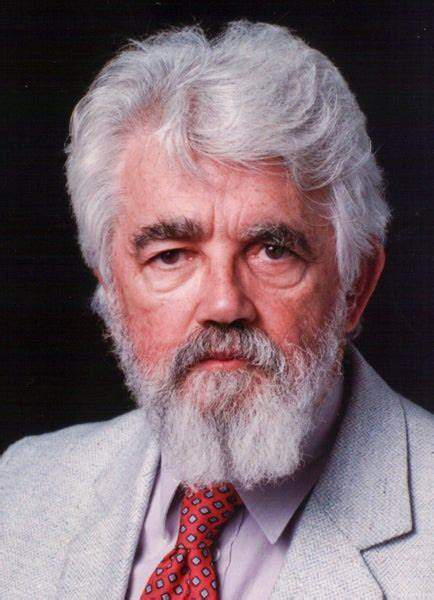
\includegraphics[width=0.20\textwidth]{John-McCarthy}}
    \hspace{0.3cm}
    \subfloat[Lisp]{
\includegraphics[width=0.25\textwidth]{LISP}}
  \end{figure}
  \begin{itemize}
  \item Family of Meta-programming languages, first specified in by John McCarthy in 1960
  \item Short for \textit{List Processing}
  \item Macros (meta-programming)
  \item Introduced garbage collection
  \item Introduced Read-Eval-Print Loop, i.e. REPL
  \item Introduced dynamic typing
  \item Introduced conditionals
  \item Introduced higher-order functions
  \item Racket, Scheme, Common Lisp, Clojure
  \end{itemize}
\end{frame}

\begin{frame}{ML}
  \begin{figure}[H]
    \centering
    \subfloat[Robin Milner, type system, ML]{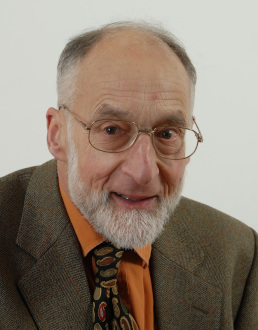
\includegraphics[width=0.15\textwidth]{Robin-Milner}}
    \hspace{0.3cm}
    \subfloat[Robert Harper, module system, SML]{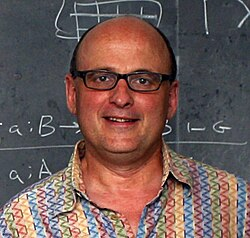
\includegraphics[width=0.15\textwidth]{Robert-Harper}}
    \hspace{0.3cm}
    \subfloat[Mads Tofte, formal definition, SML]{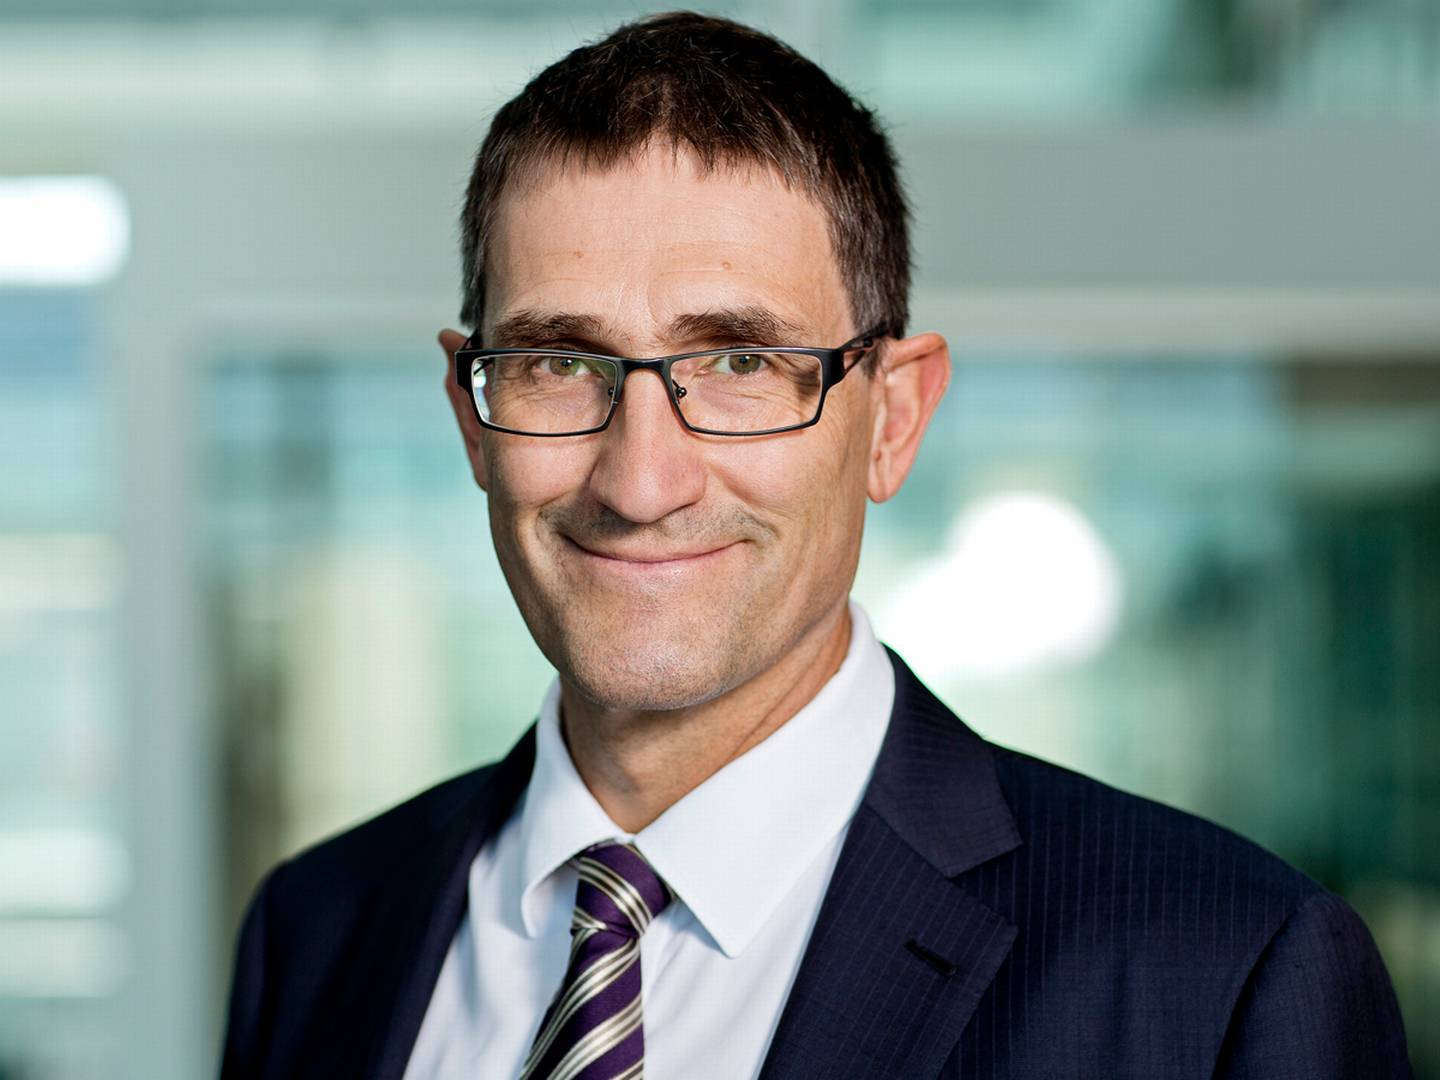
\includegraphics[width=0.15\textwidth]{Mads-Tofte}}
    \hspace{0.3cm}
    \subfloat[David MacQueen, core language, SML]{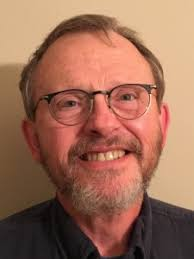
\includegraphics[width=0.15\textwidth]{David-MacQueen}}
    \hspace{0.3cm}
  \end{figure}
  \begin{itemize}
    \item Short for \emph{Meta Language}
    \item Family of strict and impure functional languages. Some implementations: SML, OCaml, F\#
    \item Introduced type inference with the Hindley-Milner type system
    \item Algebraic datatypes and pattern matching
    \item ML modules
  \end{itemize}
\end{frame}

\begin{frame}{Erlang}
  \begin{figure}[H]
    \centering
    \subfloat[Joe Armstrong]{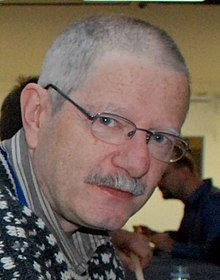
\includegraphics[width=0.15\textwidth]{Joe-Armstrong}}
    \subfloat[Robert Virding]{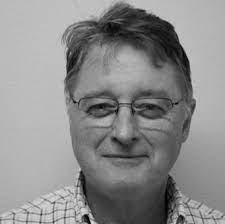
\includegraphics[width=0.15\textwidth]{Robert-Virding}}
    \subfloat[Mike Williams]{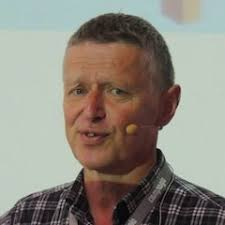
\includegraphics[width=0.15\textwidth]{Mike-Williams}}
    \hspace{0.2cm}
    \subfloat[Erlang]{
\includegraphics[width=0.25\textwidth]{Erlang}}
  \end{figure}
  \begin{itemize}
  \item Strong support for concurrency
  \item Strict and dynamically typedx
  \item Developed in 1986 at Ericsson for telecommuting purposes
  \item Named after mathematician Agner Krarup Erlang and short for \emph{Ericson Language}
  \item Hot code reloading
  \item BEAM VM
  \item REPL
  \end{itemize}
\end{frame}

\begin{frame}{Miranda}
  \begin{figure}[H]
    \centering
    \subfloat[David Turner]{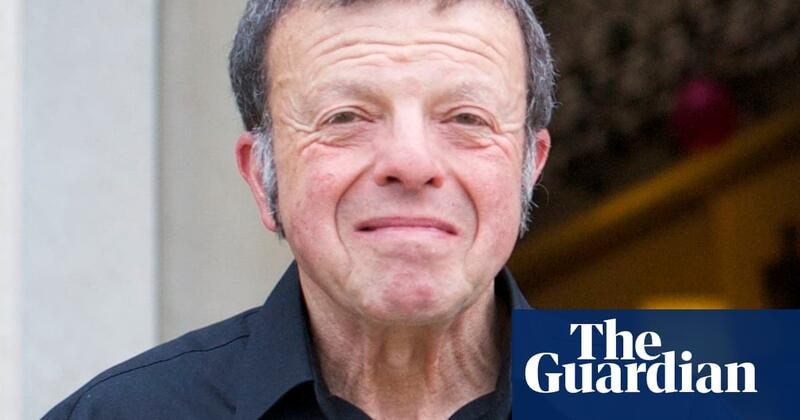
\includegraphics[width=0.40\linewidth]{David-Turner}}
    \hspace{0.3cm}
    \subfloat[Miranda]{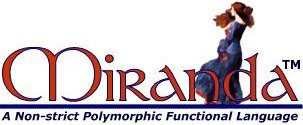
\includegraphics[width=0.33\linewidth]{Miranda}}
  \end{figure}
  \begin{itemize}
  \item Created in 1985 by David Turner
  \item Lazy and pure
  \item Algebraic datatypes
  \item Hindley-Milner type inference
  \item List comprehensions
  \end{itemize}
\end{frame}

\begin{frame}{Haskell: summary}
  \begin{figure}[H]
    \centering
    \subfloat[Haskell Curry]{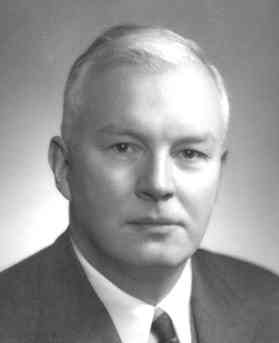
\includegraphics[width=0.20\textwidth]{Haskell-Curry}}
    \hspace{0.3cm}
    \subfloat[Haskell]{
\includegraphics[width=0.33\textwidth]{haskell-logo}}
  \end{figure}
      \begin{itemize}
      \item Lazy and pure
      \item Similar syntax to Miranda
      \item Named after logician Haskell Brooks Curry
      \item List comprehension
      \item Kind system
      \item Type inference
      \item Introduced type classes (ad-hoc polymorphism) and Monads
      \end{itemize}
\end{frame}

\begin{frame}{Haskell: history}
  \begin{figure}[H]
    \centering
    \subfloat[Working group 2.8]{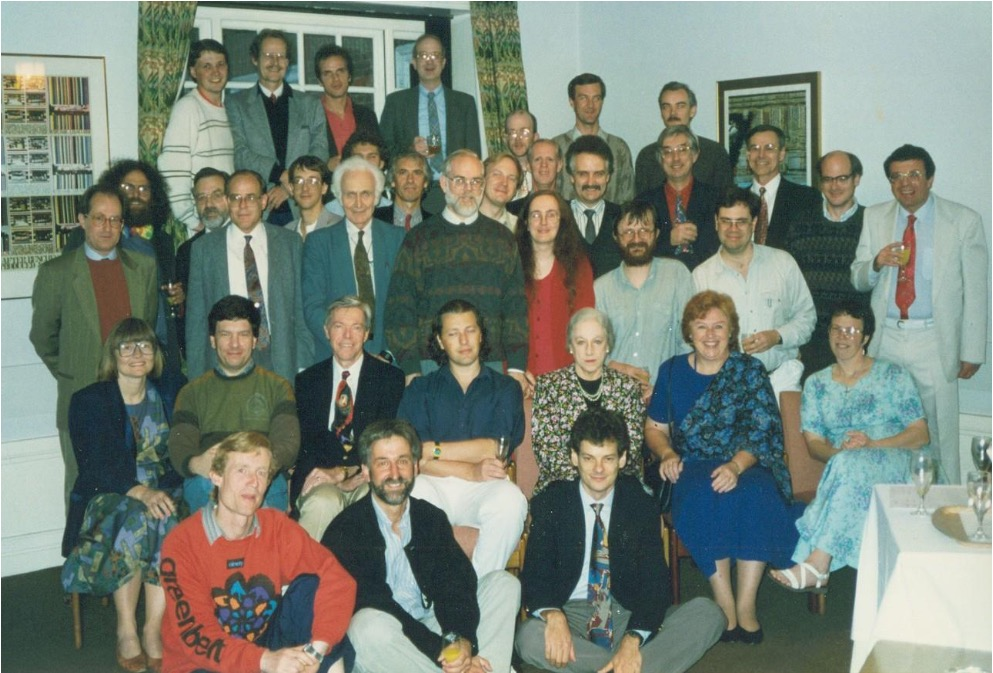
\includegraphics[width=0.33\textwidth]{haskell-working-group}}
    \begin{itemize}
    \item Devised by a committee in 1998
    \item Developed to have a single standard for \textit{pure} and \textit{lazy} functional languages
    \item Later standards Haskell98 and Haskell2010
    \end{itemize}
  \end{figure}
\end{frame}

\begin{frame}{Haskell: The original Haskell98 committee}
  \begin{figure}[H]
    \centering
    \scalebox{0.65}{%
      \begin{minipage}[c]{0.80\linewidth}
      \begin{itemize}
      \item Simon Peyton Jones, Microsoft Research, Cambridge
      \item Lennart Augustsson, Sandburst Corporation
      \item Dave Barton, Intermetrics
      \item Brian Boutel, Victoria University of Wellington
      \item Warren Burton, Simon Fraser University
      \item Joseph Fasel, Los Alamos National Laboratory
      \item Kevin Hammond, University of St. Andrews
      \item Ralf Hinze, University of Bonn
      \item Paul Hudak, Yale University
      \item John Hughes, Chalmers University of Technology
      \item Thomas Johnsson, Chalmers University of Technology
      \item Mark Jones, Oregon Graduate Institute
      \item John Launchbury, Oregon Graduate Institute
      \item Erik Meijer, Microsoft Corporation
      \item John Peterson, Yale University
      \item Alastair Reid, University of Utah
      \item Colin Runciman, York University
      \item Philip Wadler, Avaya Labs
      \end{itemize}
    \end{minipage}}

  \end{figure}
  \end{frame}

  \begin{frame}{Haskell: Some of the influential people throughout the years}

      {\small Simon Peyton Jones, Philip Wadler, Stephenie Weirich, Richard Eisenberg, Arvind, Lennart Augustsson, Dave Barton, Brian Boutel, Warren Burton, Manuel M T Chakravarty, Duncan Coutts, Jon Fairbairn,Joseph Fasel, John Goerzen,Andy Gordon, Maria Guzman, Kevin Hammond, Bastiaan Heeren, Ralf Hinze, Paul Hudak, John Hughes, Thomas Johnsson, Isaac Jones, Mark Jones, Dick Kieburtz, John Launchbury, Andres Löh, Ian Lynagh, Simon Marlow, John Meacham, Erik Meijer, Ravi Nanavati, Rishiyur Nikhil, Henrik Nilsson, Ross Paterson, John Peterson, Mike Reeve, Alastair Reid, Vladislav Zaviolav, Ryan Scott, Colin Runciman, Don Stewart, Martin Sulzmann, Audrey Tang, Simon Thompson, Malcolm Wallace, David Wise, Jonathan Young, and many more!}
\end{frame}

\begin{frame}{Haskell: implementations}
  \begin{itemize}
  \item GHC
  \item hbc
  \item hugs
  \item Yale Haskell
  \item UHC
  \item LHC
  \end{itemize}

\end{frame}

\begin{frame}{GHC Haskell}
  \begin{figure}[H]
    \centering
    \subfloat[Simon Peyton Jones]{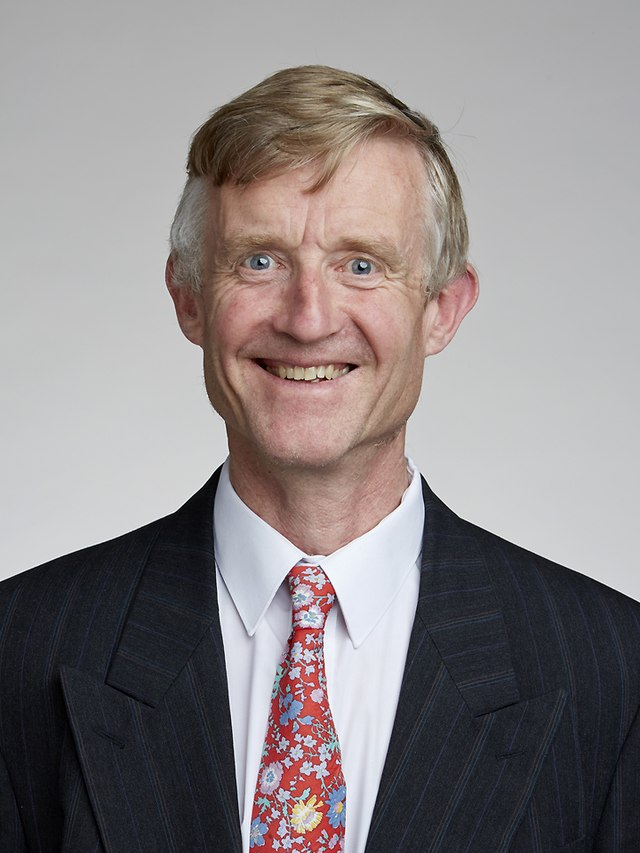
\includegraphics[width=0.22\textwidth]{Simon-Peyton-Jones}}
    \hspace{0.2cm}
    \subfloat[Simon Marlow]{{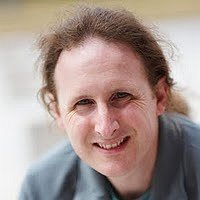
\includegraphics[width=0.22\textwidth]{Simon-Marlow}}}
    \caption{Original authors of GHC}
  \end{figure}

  Some of the features of GHC:
  {\small Impredicativity, GADTs, Existential types, Type families,
  Type abstractions, Required type arguments ,Pattern synonyms, Higher-Rank types, Kind polymorphism,
  Dependent kinds and ...!}
\end{frame}

\begin{frame}{GHCi: GHC's REPL}
  \begin{figure}[H]
    \centering
    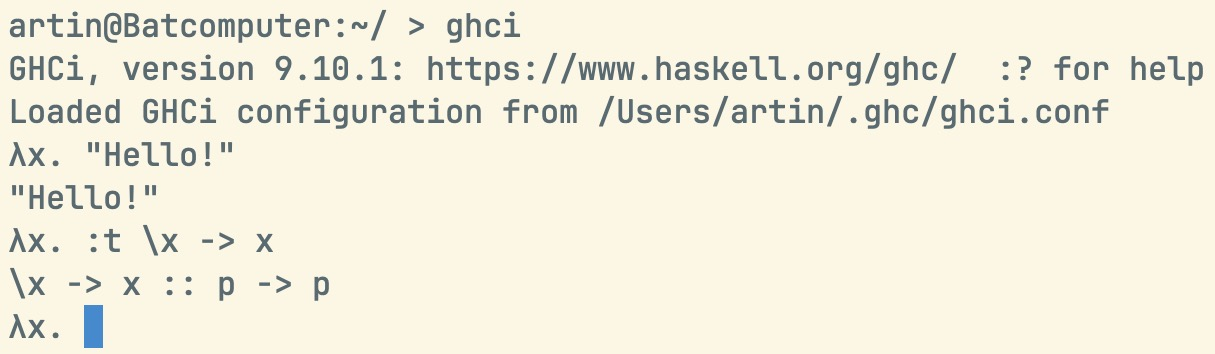
\includegraphics[width=0.50\textwidth]{ghci}
  \end{figure}
  \begin{itemize}
  \item GHC has a REPL called GHCi that let's you compile Haskell to byte code and run it interactively.
  \item You can ask for the type of something in GHCi by using the \code{:t} command
  \end{itemize}
\end{frame}

\begin{frame}{Defining functions}
  \begin{figure}[H]
    \centering
    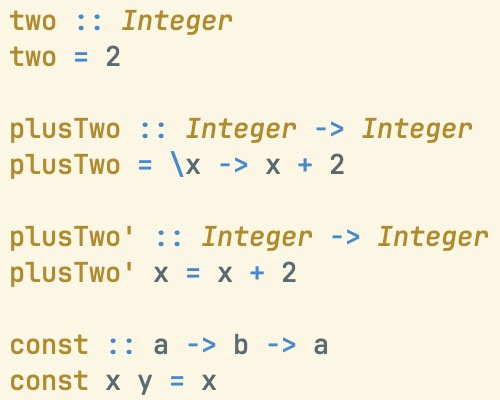
\includegraphics[width=0.50\textwidth]{decls}
  \end{figure}
  \begin{itemize}
    \item The part with \code{::} is called the \emph{type signature} of the function
    \item The part with \code{=} is called the \emph{function defintion} or the \emph{function equation}
  \end{itemize}
\end{frame}

\begin{frame}{Using functions}
  Just like in Lambda-calculus, in order to apply a function to its argument, we don't need to put the arguments in parenthesis.

  Applying the function \code{f} to arguments \code{x} and {y}:
  \begin{itemize}
  \item Python: \code{f(x,y)}
  \item Haskell: \code{f x y}
  \item Lambda-Calculus: \code{f x y}
  \end{itemize}
\end{frame}

\begin{frame}{Operators are functions too}
  \begin{figure}[H]
    \centering
    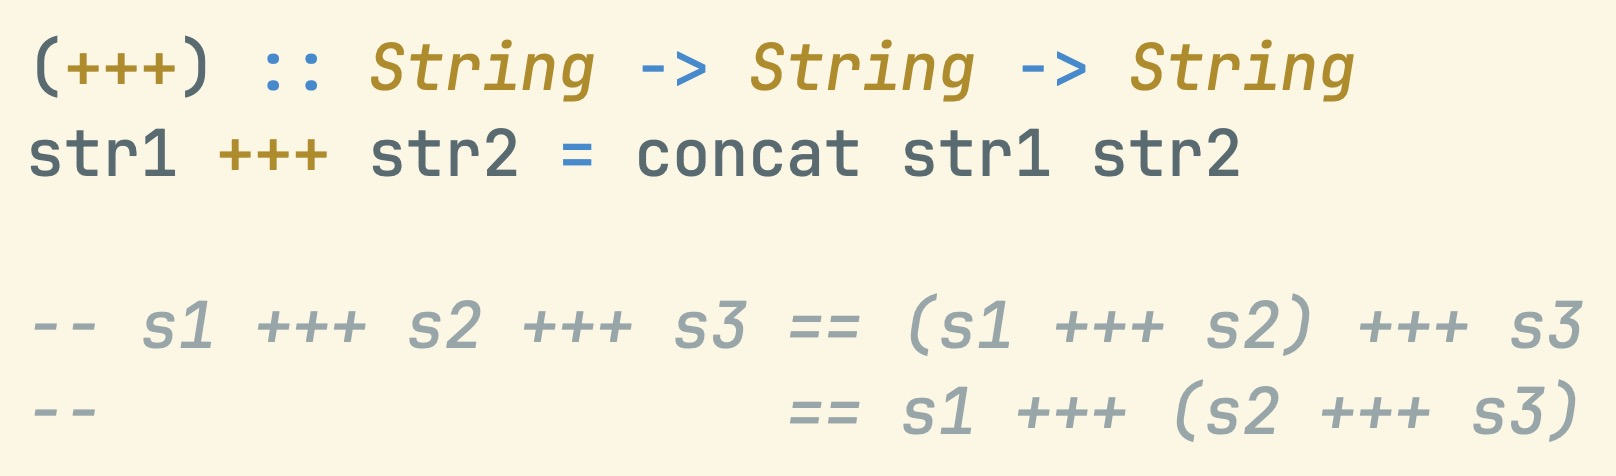
\includegraphics[width=\textwidth]{concat-op}
  \end{figure}
  \begin{itemize}
  \item Easier to chain together
  \item Easier to show algebraic laws like associativity
  \end{itemize}
\end{frame}

\begin{frame}{Function composition}
  \begin{itemize}
  \item Just another function!
  \item Takes to functions and a value. First applies the second argument and then the first
  \item The \code{.} operator is amongst the most used operators!
  \end{itemize}

  \begin{figure}[H]
    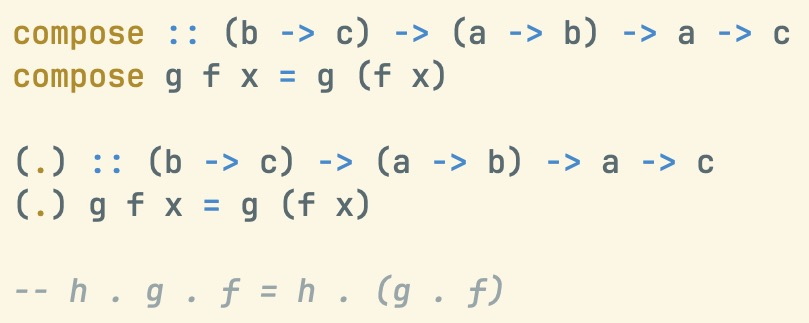
\includegraphics[width=\textwidth]{compose}
  \end{figure}
\end{frame}

\begin{frame}{Function composition: example}
  \code{\textbackslash $x \to x * 3$} is the same thing as \code{(* 3)}.
  \begin{figure}[H]
    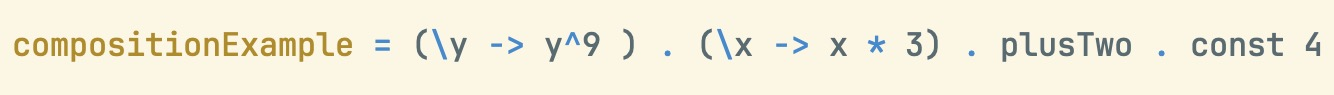
\includegraphics[width=1.0\textwidth]{compositionExample}
    \vspace{0.2cm}
    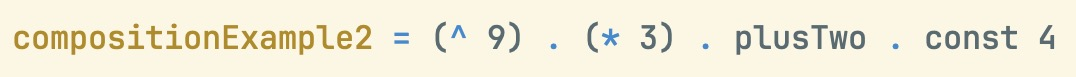
\includegraphics[width=1.0\textwidth]{compositionExample2}
    \vspace{0.2cm}
    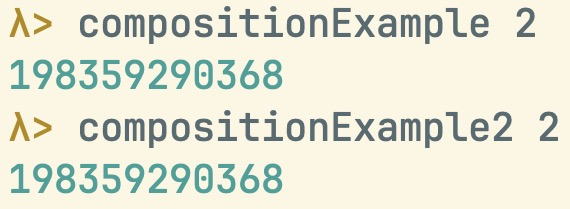
\includegraphics[width=0.70\textwidth]{compositionExample-ghci}
  \end{figure}
\end{frame}

\begin{frame}{List and laziness}
  \begin{figure}[H]
    \centering
    \subfloat[]{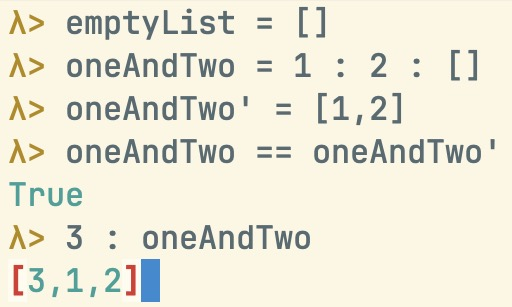
\includegraphics[width=0.50\textwidth]{emptyList-oneAndTwo}}
    \vspace{0.2cm}
    \subfloat[]{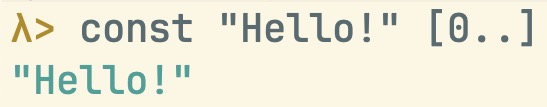
\includegraphics[width=0.50\textwidth]{const-hello-infinite}}
  \end{figure}
\end{frame}

\begin{frame}{Algebraic Datatypes}
  Algebraic Data Types are created by the combination of:
  \begin{itemize}
  \item Sum types i.e. better enums
  \item Product types i.e. better structs
  \end{itemize}

  Examples:
  \begin{itemize}
  \item Sum type: \code{Bool} is \textit{either} \code{True} or \code{False}
  \item Product type: The 2-tuple \code{(Int,String)} needs both an \code{Int} and a \code{String}. \code{(3, "Hi!""}
  \end{itemize}
\end{frame}

\begin{frame}{Algebraic Datatypes: \code{Food} type}
  \begin{figure}[H]
    \centering
    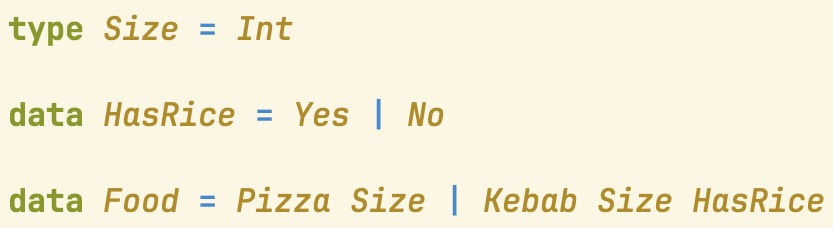
\includegraphics[width=0.80\textwidth]{food-type}
  \end{figure}
  \begin{figure}[H]
    \centering
    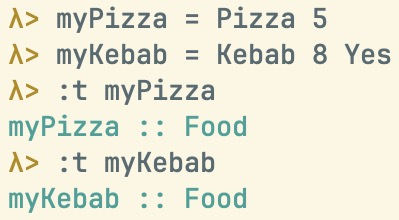
\includegraphics[width=0.40\textwidth]{food-example}
  \end{figure}
  \code{Food} has two \emph{data constructors}:
  \begin{itemize}
  \item \code{Pizza}: In order to make \code{Pizza} you need to give it a value of type \code{Size}
  \item \code{Kebab}: In order to make \code{Kebab} you need to give it a value of type \code{Size} \textbf{and} a value of type \code{HasRice}
  \end{itemize}
\end{frame}

\begin{frame}{Pattern matching}
  You can \emph{match} and \emph{deconstruct} patterns on the left hand side of an equation

    \begin{figure}[H]
    \centering
    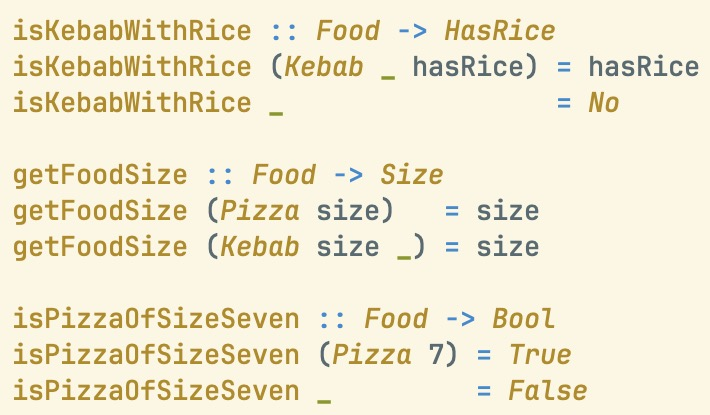
\includegraphics[width=0.60\textwidth]{food-pattern-match}
  \end{figure}

  \begin{itemize}
  \item Patterns can \emph{deconstruct} data constructors, \emph{introduce} variables, or always match by having a \emph{wildcard}
  \item Patterns can be as nested as you want!
  \end{itemize}
\end{frame}

\begin{frame}{The \code{map} function}
  The \code{map} function applies a function to all of the elements of a list

  Examples
\begin{figure}[H]
    \centering
    \subfloat[Example 1]{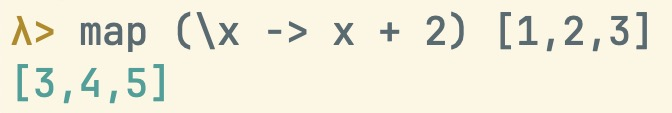
\includegraphics[width=\textwidth]{map-x-plus-two}}
    \vspace{0.1cm}
    \subfloat[Example 2]{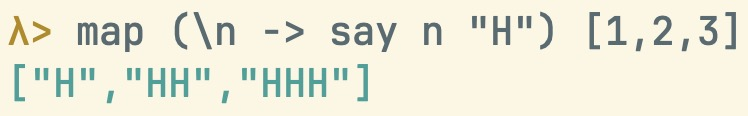
\includegraphics[width=\textwidth]{map-say}}
    \vspace{0.1cm}
    \pause
  \end{figure}
\end{frame}

\begin{frame}{The \code{map} function in action}
  \begin{figure}[H]
    \centering
    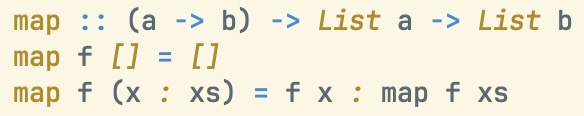
\includegraphics[width=\textwidth]{map-hs}
  \end{figure}
  Important Note: Because of laziness, Haskell doesn't actually reduce the applications until it's needed!

  Let's evaluate \code{map (+2) [1,2,3]}
  \begin{enumerate}
  \item \code{map (+2) [1,2,3]}
  \item \code{(1 + 2) : map (+2) [2,3]}
  \item \code{(1 + 2) : (2 + 2) : map (+2) [3]}
  \item \code{(1 + 2) : (2 + 2) : (3 + 3) : map (+2) []}
  \item \code{(1 + 2) : (2 + 2) : (3 + 2) : []}
  \item \code{3 : 4 : 5 : []}
  \item \code{[3,4,5]}
  \end{enumerate}
\end{frame}

\begin{frame}{The \code{Maybe} type and its usage}
  \begin{figure}[H]
    \centering
    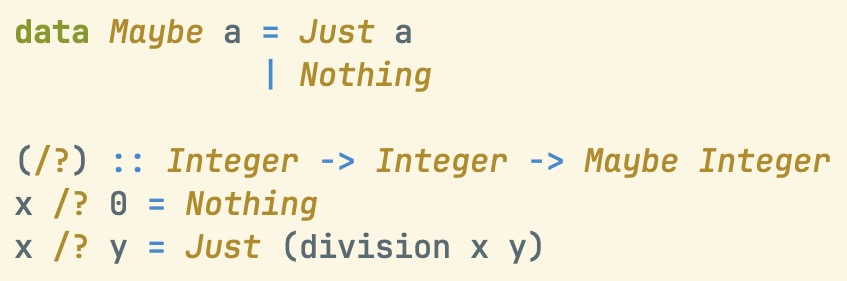
\includegraphics[width=0.70\textwidth]{Maybe-hs}
  \end{figure}
  Why is this better than throwing an error?
  \begin{itemize}
  \item Errors are thrown when we \textit{run} the program. We want the compiler to catch the bug during \textit{compilation}!
  \item By reading the type of \code{$(/?)$} i.e. \code{$Integer \to Integer \to Maybe Integer$}, we find out that this function could \textit{fail}
  \end{itemize}
\end{frame}

\begin{frame}{The \code{Maybe} type and its usage}
  Important note: GHCi compiles the code before running it
\begin{figure}[H]
    \centering
    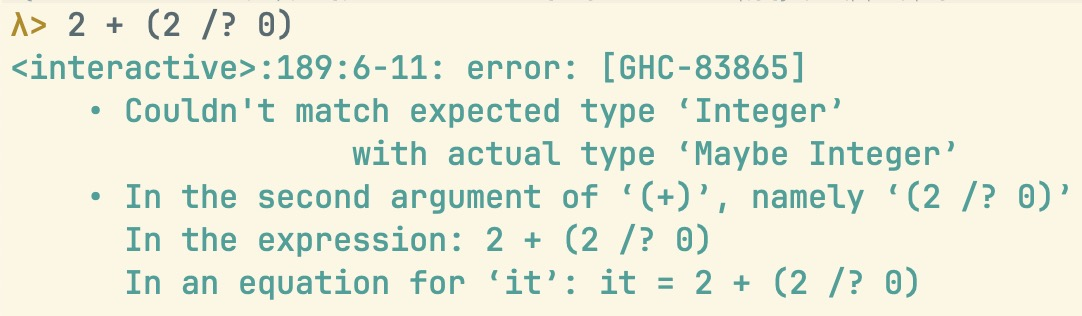
\includegraphics[width=\textwidth]{safeDivision}
  \end{figure}
\end{frame}

\begin{frame}{Type classes: Ad-hoc polymorphism}
  Type classes give us access to ad-hoc polymorphism.

  As an example, The \code{Show} type class lets us convert values into strings.
  \begin{figure}[H]
    \centering
    \subfloat[]{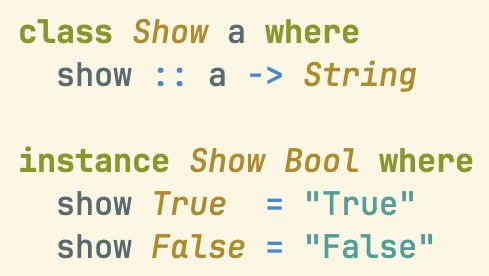
\includegraphics[width=0.45\textwidth]{show-class}}
    \hspace{0.1cm}
    \subfloat[]{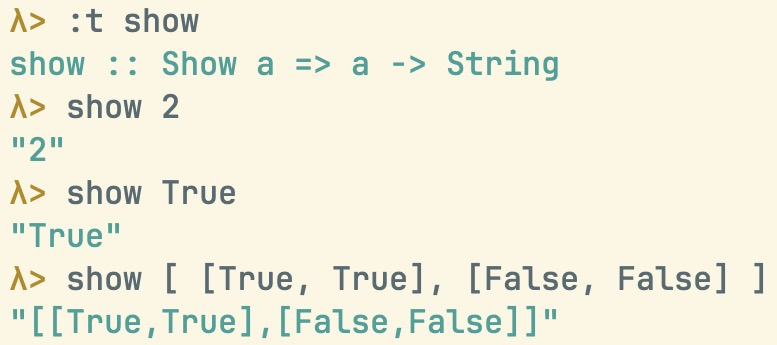
\includegraphics[width=0.50\textwidth]{show-examples}}
  \end{figure}
\end{frame}

\begin{frame}{Type classes: Deriving}
  Haskell can write \emph{most} of the type class instances for you!
  \begin{figure}[H]
    \centering
    \subfloat[\code{Day} type]{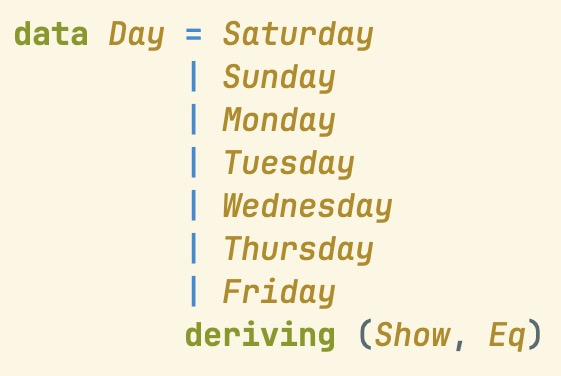
\includegraphics[width=0.50\textwidth]{deriving-day}}
    \hspace{0.3cm}
    \subfloat[Examples in GHCi]{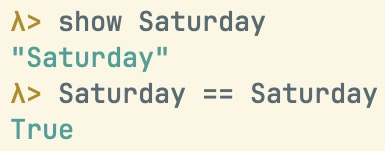
\includegraphics[width=0.50\textwidth]{derived-show-day-ghci}}
  \end{figure}
\end{frame}

\begin{frame}{Datatypes as contexts}
  \begin{itemize}
  \item List: Order matters
  \item Tree: Easy navigation and lookup
  \item Maybe: Computation could fail
  \end{itemize}

  All of these have one thing in common: They all hold values inside them, and you can see the type of that value from outside.
  \begin{itemize}
  \item \code{Maybe String} holds a value of type \code{String}
  \item \code{List a} holds values of type \code{a}
  \item \code{Tree Food} holds values of type \code{Food}
  \end{itemize}

\end{frame}

\begin{frame}{The \code{Functor} class}
  \begin{figure}[H]
    \centering
    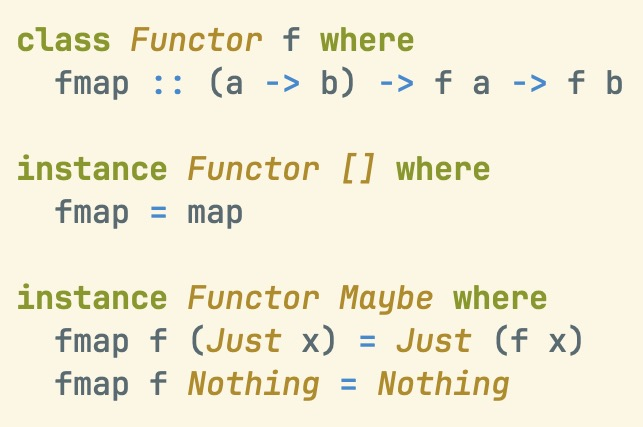
\includegraphics[width=0.80\textwidth]{functor-class}
  \end{figure}
  Laws:
  \begin{itemize}
  \item \code{$fmap \: (g \circ f) \: x \equiv (fmap \: g \circ fmap \: f) \: x$}
  \item \code{$fmap \: id \: x \equiv x$}
  \end{itemize}
\end{frame}

\begin{frame}{Functor: examples}
  \begin{figure}[H]
    \centering
    \subfloat[]{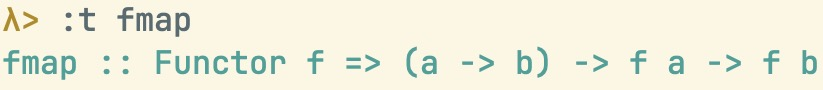
\includegraphics[width=0.80\textwidth]{type-of-fmap}}
    \hspace{0.2cm}
    \subfloat[]{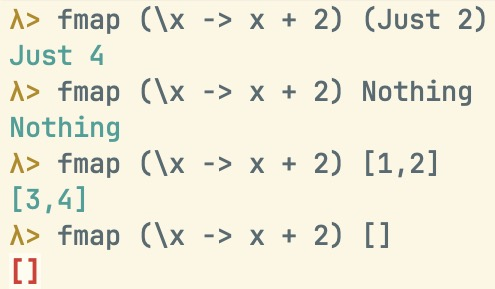
\includegraphics[width=0.80\textwidth]{functor-examples}}
  \end{figure}
\end{frame}

\section{Types}
\label{sec:types}

\begin{frame}[fragile]{Type Inference}
  \begin{figure}[H]
    \centering
    \subfloat[]{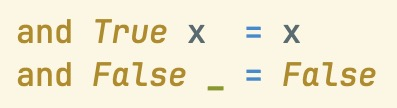
\includegraphics[width=0.45\textwidth]{and-no-sig}}
    \hspace{0.1cm}
    \subfloat[]{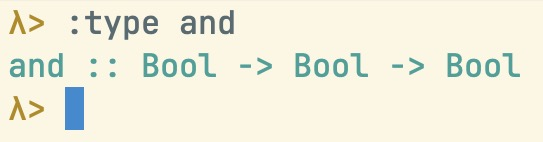
\includegraphics[width=0.45\textwidth]{type-of-and}}
  \end{figure}
  Haskell is smart enough to \textit{infer} the type of most functions by itself. And if you give it the wrong argument, it will tell you exactly what you did wrong!

  e.g. \code{test = and True 'c'} will result in the following error message:
  \begin{figure}[H]
    \centering
    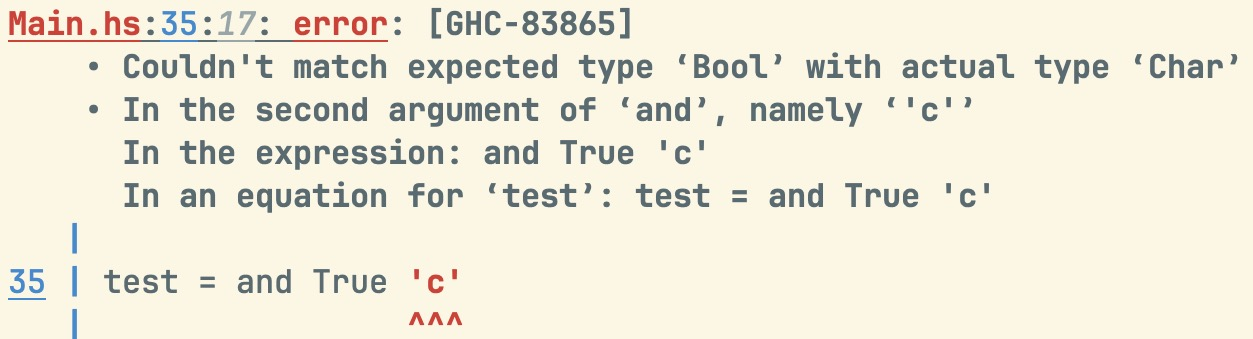
\includegraphics[width=\linewidth]{and-type-error}
  \end{figure}
\end{frame}
\begin{frame}[fragile]{Type Inference}
  \begin{figure}[H]
    \centering
    \subfloat[]{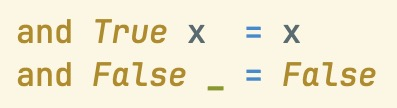
\includegraphics[width=0.45\textwidth]{and-no-sig}}
    \hspace{0.1cm}
    \subfloat[]{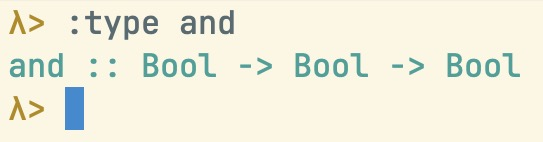
\includegraphics[width=0.45\textwidth]{type-of-and}}
  \end{figure}
  Haskell is smart enough to \textit{infer} the type of most functions by itself. And if you give it the wrong argument, it will tell you exactly what you did wrong!

  e.g. \code{test = and True 'c'} will result in the following error message:
  \begin{figure}[H]
    \centering
    \includegraphics[width=\linewidth]{and-type-error}
  \end{figure}
\end{frame}

\begin{frame}{Type Inference}
  TODO rephrase Haskell's type system is so clever that we didn't need \emph{any} type signatures for the examples I showed you!
  Because of this, the type signature of the upcoming examples are commented out.

  Here are some reasons for why you should write them though:
  \begin{itemize}
  \item Type signatures are like documentation, they tell us a lot about the function at hand
  \item Sometimes Haskell infers types that are \emph{more} polymorphic than you'd want
  \item When refactoring, you might unknowingly change the type of functions
  \end{itemize}
\end{frame}

\begin{frame}{Example: \code{factorial} in Python}
  \begin{figure}[H]
    \centering
    \includegraphics[width=\linewidth]{factorial-py}
  \end{figure}
\end{frame}

\begin{frame}{Example: \code{factorial} in Haskell}
    \begin{figure}[H]
    \centering
    \includegraphics[width=\linewidth]{factorial-hs}
  \end{figure}

  \pause
  Let's evaluate \code{factorial 3}:

  \begin{enumerate}
    \item<1-> \code{factorial 3}
    \item<2-> \code{3 * factorial 2}
    \item<3-> \code{3 * 2 * factorial 1}
    \item<4-> \code{3 * 2 * 1 * factorial 0}
    \item<5-> \code{3 * 2 * 1 * 1}
    \item<6-> \code{6 * 1 * 1}
    \item<7-> \code{6 * 1}
    \item<8-> \code{6}
  \end{enumerate}

\end{frame}

\begin{frame}{Example: \code{say} in Python}

  \code{say} is a function that given a number \textit{n} and a string \textit{string}, will repeat the \textit{string} \textit{n} times.

  e.g. \code{say(2,"Hi ") = "Hi Hi "}

  \begin{figure}[H]
    \centering
    \includegraphics[width=\linewidth]{say-py}
  \end{figure}

\end{frame}

\begin{frame}{Example: \code{say} in Haskell}
  The \code{++} operator concatenates two strings together.

  \begin{figure}[H]
    \centering
    \includegraphics[width=\linewidth]{say-hs}
  \end{figure}

  \pause
  Let's evaluate \code{say 2 "Hi "}:

  \begin{enumerate}
    \item<1-> \code{say 2 "Hi "}
    \item<2-> \code{"Hi " ++ say 1 "Hi"}
    \item<3-> \code{"Hi " ++ "Hi " ++ say 0 "Hi"}
    \item<4-> \code{"Hi " ++ "Hi " ++ ""}
    \item<5-> \code{"Hi Hi " ++ ""}
    \item<6-> \code{"Hi Hi "}
  \end{enumerate}

\end{frame}

\begin{frame}[fragile]{Example: \code{hasEven} in Python}
  \code{hasEven} is a function that given a character, \textit{char}
  ,and a string \textit{string}, will return \textit{true} if the number
  of times \textit{char} occurs in \textit{string} is even.

  \begin{figure}[H]
    \centering
    \includegraphics[width=\linewidth]{hasEven-py}
  \end{figure}

\end{frame}

\begin{frame}{Example: \code{hasEven} in Haskell}
  \code{even} is a built-in function that says whether its input is even or not.
    \begin{figure}[H]
    \centering
    \includegraphics[width=\linewidth]{hasEven-hs}
  \end{figure}
\end{frame}

\begin{frame}{Example: \code{hasEven} in Haskell}
    \begin{figure}[H]
    \centering
    \includegraphics[width=0.80\linewidth]{hasEven-hs}
  \end{figure}

  \pause
  Let's evaluate \code{hasEven 'e' "eyes"}:

  \begin{enumerate}
    \item<1-> \code{even (loop 0 "eyes")}
    \item<2-> \code{even (loop 1 "yes")}
    \item<3-> \code{even (loop 1 "es")}
    \item<4-> \code{even (loop 2 "s")}
    \item<5-> \code{even (loop 2 "")}
    \item<6-> \code{even 2}
    \item<7-> \code{True}
  \end{enumerate}

\end{frame}

\section{Influence of functional languages on imperative languages}
\label{sec:influence}

\begin{frame}{Python}
  \begin{itemize}
  \item Lambdas
  \item Dynamic Typing
  \item Garbage collection
  \item List comprehension
  \end{itemize}
\end{frame}

\begin{frame}{Excel}
  As unbelievable as it is, Excel has become turing complete!

  Simon Peyton Jones (Haskell) and Andy Gordon have added lambdas to Excel in 2021
\end{frame}

\begin{frame}{Rust}
  \begin{itemize}
  \item Anonymous functions
  \item Traits, which are the equivalents of Haskell's type classes
  \item Prioritizing immutability
  \item Pattern matching
  \item The type system itself is inspired on ML
  \item Macros which are the same as Scheme's macro system
  \end{itemize}
\end{frame}

\begin{frame}{Swift}
  \begin{itemize}
  \item SwiftUI, apple's UI library is incredibly composable and
  \item Closures, which are close to lambdas
  \item Syntactic sugar for closures
  \item Enums and structs are algebraic datatypes!
  \item Pattern matching
  \item Optional chaining is based on the idea of Monads!
  \end{itemize}
\end{frame}

\begin{frame}{Java}
  \begin{itemize}
  \item \item Lambdas
  \item Java's generics was designed by Philip Wadler (Haskell) himself!
  \item Pattern matching
  \end{itemize}
\end{frame}

\begin{frame}{React}
  React is heavily based on functional programming ideas like pure functions, immutability, avoiding mutation, and avoiding state!
\end{frame}

\begin{frame}{In industry}
  \begin{itemize}
  \item NASA' copilot and ogma projects are written in Haskell
  \item Meta's spam filter is written in Haskell
  \item JP Morgan uses Haskell
  \item IOHK cardano uses Haskell
  \item Siemens uses Haskell
  \item Jane Street uses OCaml
  \item Epic Games is developing Verse to use in its metaverse
  \item X's backend is written Scala
  \item Spotify's backend is written in Scala
  \item Whatsapp is written in Erlang
  \item Discord is written in Elixir
  \item Tesla uses Haskell to generate C code for its cars
  \item And many more!
  \end{itemize}
\end{frame}

\begin{frame}{More functional languages}
  \begin{itemize}
  \item Idris2
  \item Flix
  \item Lean4
  \item OCaml
  \item Verse
  \item Racket
  \item Janet
  \item Common Lisp
  \item Scheme
  \item Clojure
  \item Gleam
  \item Scala
  \item Elixir
  \item OCaml
  \item F\#
  \end{itemize}
\end{frame}

\end{document}
